\documentclass[12pt,a4paper]{article}

\usepackage{fontawesome5}
\providecommand{\faPencilAlt}{\faIcon{pencil-alt}}

\usepackage{styles/couleurs}
\usepackage{styles/mise_en_page}
\usepackage{styles/boites}
\usepackage{styles/maths}
\usepackage{styles/figures}

\usepackage{enumitem}
\usepackage{array}
\usepackage{tabularx}
\usepackage{amsmath}
\usepackage{amssymb}
\usepackage{graphicx}
\usepackage{tikz}
\usepackage{xparse}

\usetikzlibrary{calc,arrows.meta}

\setlist[itemize]{leftmargin=1.4em,itemsep=0.15em,topsep=0.2em}
\setlist[enumerate]{leftmargin=*,itemsep=0.22em,topsep=0.25em}

\newcommand{\lignepointillee}{%
  \noindent\dotfill\par
  \vspace{0.45em}
}

\newcommand{\lignesreponse}[1]{%
  \begin{tcolorbox}[
    enhanced,
    colback=white,
    colframe=NeutreC!40,
    boxrule=0.5pt,
    arc=1.5mm,
    left=3mm,
    right=3mm,
    top=2mm,
    bottom=1mm,
    before skip=2pt,
    after skip=2pt
  ]
    \foreach \i in {1,...,#1}{\lignepointillee}
  \end{tcolorbox}
}

\newcommand{\imageactivite}[3]{%
  \IfFileExists{#3}{%
    \includegraphics[width=#1,height=#2,keepaspectratio]{#3}%
  }{%
    \fbox{%
      \parbox[c][#2][c]{#1}{%
        \centering\sffamily\small
        Image à intégrer\par
        \vspace{0.3em}
        \texttt{\detokenize{#3}}
      }%
    }%
  }%
}

\newcommand{\titreseq}[1]{%
\begin{center}
  {\sffamily\LARGE\bfseries\color{TitreC}
  Séquence 5 -- Statistiques et proportionnalité}\\[0.2em]
  {\sffamily\large\bfseries\color{SavoirC}#1}
\end{center}
}

\begin{document}

\titreseq{Activité 7 -- Construire un diagramme circulaire}

On reprend l'enquête sur les \(40\) élèves.

\[
\begin{array}{c|cccc}
\text{Mode de transport} & \text{Bus} & \text{À pied} & \text{Voiture} & \text{Vélo}\\
\hline
\text{Effectif} & 16 & 10 & 8 & 6
\end{array}
\]

\section*{Partie A -- Du total au cercle entier}

Un cercle entier mesure \(360^\circ\).

Complète :

\[
40\text{ élèves}\longleftrightarrow360^\circ
\]

\[
1\text{ élève}\longleftrightarrow\ldots^\circ
\]

Quelle opération permet de passer d'un effectif à l'angle correspondant ?

\lignesreponse{3}

\section*{Partie B -- Compléter le tableau}

\renewcommand{\arraystretch}{1.55}
\begin{tabularx}{\textwidth}{
|>{\raggedright\arraybackslash}p{3cm}
|>{\centering\arraybackslash}X
|>{\centering\arraybackslash}X
|>{\centering\arraybackslash}X
|>{\centering\arraybackslash}X
|>{\centering\arraybackslash}X|}
\hline
 & \textbf{Bus} & \textbf{À pied} & \textbf{Voiture} & \textbf{Vélo} & \textbf{Total}\\
\hline
\textbf{Effectif} & 16 & 10 & 8 & 6 & 40\\
\hline
\textbf{Pourcentage} & & & & & \(100\%\)\\
\hline
\textbf{Angle} & & & & & \(360^\circ\)\\
\hline
\end{tabularx}

Vérifie que la somme des angles vaut \(360^\circ\).

\section*{Partie C -- Construire}

\begin{center}
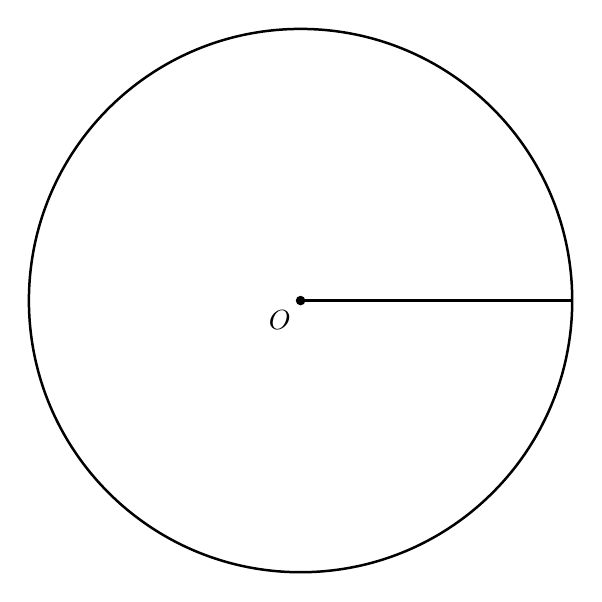
\begin{tikzpicture}[scale=1.15]
  \draw[line width=0.9pt] (0,0) circle (3);
  \draw[line width=0.9pt] (0,0)--(3,0);
  \fill (0,0) circle (1.5pt);
  \node[below left] at (0,0) {\(O\)};
\end{tikzpicture}
\end{center}

À l'aide du rapporteur :

\begin{enumerate}
  \item construis les secteurs les uns après les autres ;
  \item colorie-les ou utilise des hachures différentes ;
  \item ajoute une légende et un titre ;
  \item indique la source et l'effectif total.
\end{enumerate}

\section*{Partie D -- Contrôler}

Explique comment vérifier le diagramme sans recommencer toute la construction.

\lignesreponse{4}

\end{document}
